\section{Classifier}

\subsection{Architecture}
We explored different architectures for the convolutional neural network (CNN) for split error detection. We compare traditional CNN architectures versus residual networks~\cite{resnet} (Tab.~\ref{tab:architecture}). The traditional architecture with dropout regularization generalized better than residual networks on unseen testing data.

\begin{table}[t]
\caption{Traditional CNN Architecture versus Residual Network Architecture \cite{resnet}. All configurations are compared using the same parameters. Our final choice (indicated by *) trains relatively fast and performs better.}%While the training of our classifier is more expensive, testing accuracy is superior. }

\small{
\begin{tabular}{@{}ll|l@{}}
	\toprule
     ~ & \textbf{Traditional Network} & \textbf{Residual Network}  \\ \midrule	
\begin{tabular}{@{}r|@{}}
Conv. Layers \\
Dropout Reg. \\
Cost [m] \\
Test. Acc. \\
Prec./Recall \\
F1 Score\\
~
\end{tabular} & 
\begin{tabular}{@{}c|c@{}}
 2 & 4 \\
 y & y \\
 27.5 & 383 \\
 0.925 & 0.94 \\
 0.93/0.93 &
 0.94/0.94 \\
 0.93 & 0.94 \\
 ~&*
\end{tabular}
& 
\begin{tabular}{@{}c|c@{}}
 5 & 13 \\
 y & n \\
5080 & 1094 \\
 0.93 & 0.90 \\
 0.7/0.53 &
 0.74/0.66 \\
 0.39 & 0.64\\
 ~&~

\end{tabular}

\end{tabular}
\hspace{2mm}
\hrule
}
\label{tab:architecture}
\end{table}




\subsection{Training Parameters}

We performed a limited brute force parameter search to tune the split error classifier (Tab.~\ref{tab:parametersearch}). This resulted in 3240 different CNN configurations which were evaluated on 10\% of our training data. Learning rate and momentum ranges are defined linearly across 2000 epochs.

\begin{table}[t]
\caption{Brute force parameter search for the split error classifier. The final parameters are highlighted.}%While the training of our classifier is more expensive, testing accuracy is superior. }

\small{
\begin{tabular}{@{}ll}
	\toprule
     \textbf{Parameter} & \textbf{Search Space}  \\ \midrule	
\begin{tabular}{@{}l@{}}
Filter size: \\
No. Filters 1: \\
No. Filters 2-4: \\
Dense units:\\
Learning rate: \\
Momentum: \\
Mini-Batchsize: 
\end{tabular} & 
\begin{tabular}{@{}l@{}}
\textbf{3x3}, 5x5, 9x9, 13x13\\
32, 48, \textbf{64} \\
32, \textbf{48}, 64 \\
256, \textbf{512} \\
0.00001, 0.0001, 0.001, 0.01, \textbf{0.03-0.00001} \\
0.9, 0.95, \textbf{0.9-0.999} \\
10, 100, \textbf{128}
\end{tabular}

\end{tabular}
\hspace{2mm}
\hrule
}
\label{tab:parametersearch}
\end{table}

\subsection{Automatic Method Threshold $p_t$}
For automatic selection, we observed a threshold $p_t=0.95$ as stable when evaluating on previously unseen testing data (Mouse S1 AC3 Open Connectome Project dataset). This means that automatic selection stops once all borders with $p_t\geq0.95$ were proofread. Figure~\ref{fig:cylboxplot} shows split error classification on three randomly selected subvolumes ($700\times700\times2$ voxels) of AC3. In all cases, the threshold $p_t=0.95$ reduces VI.

\begin{figure}[t]
\centering
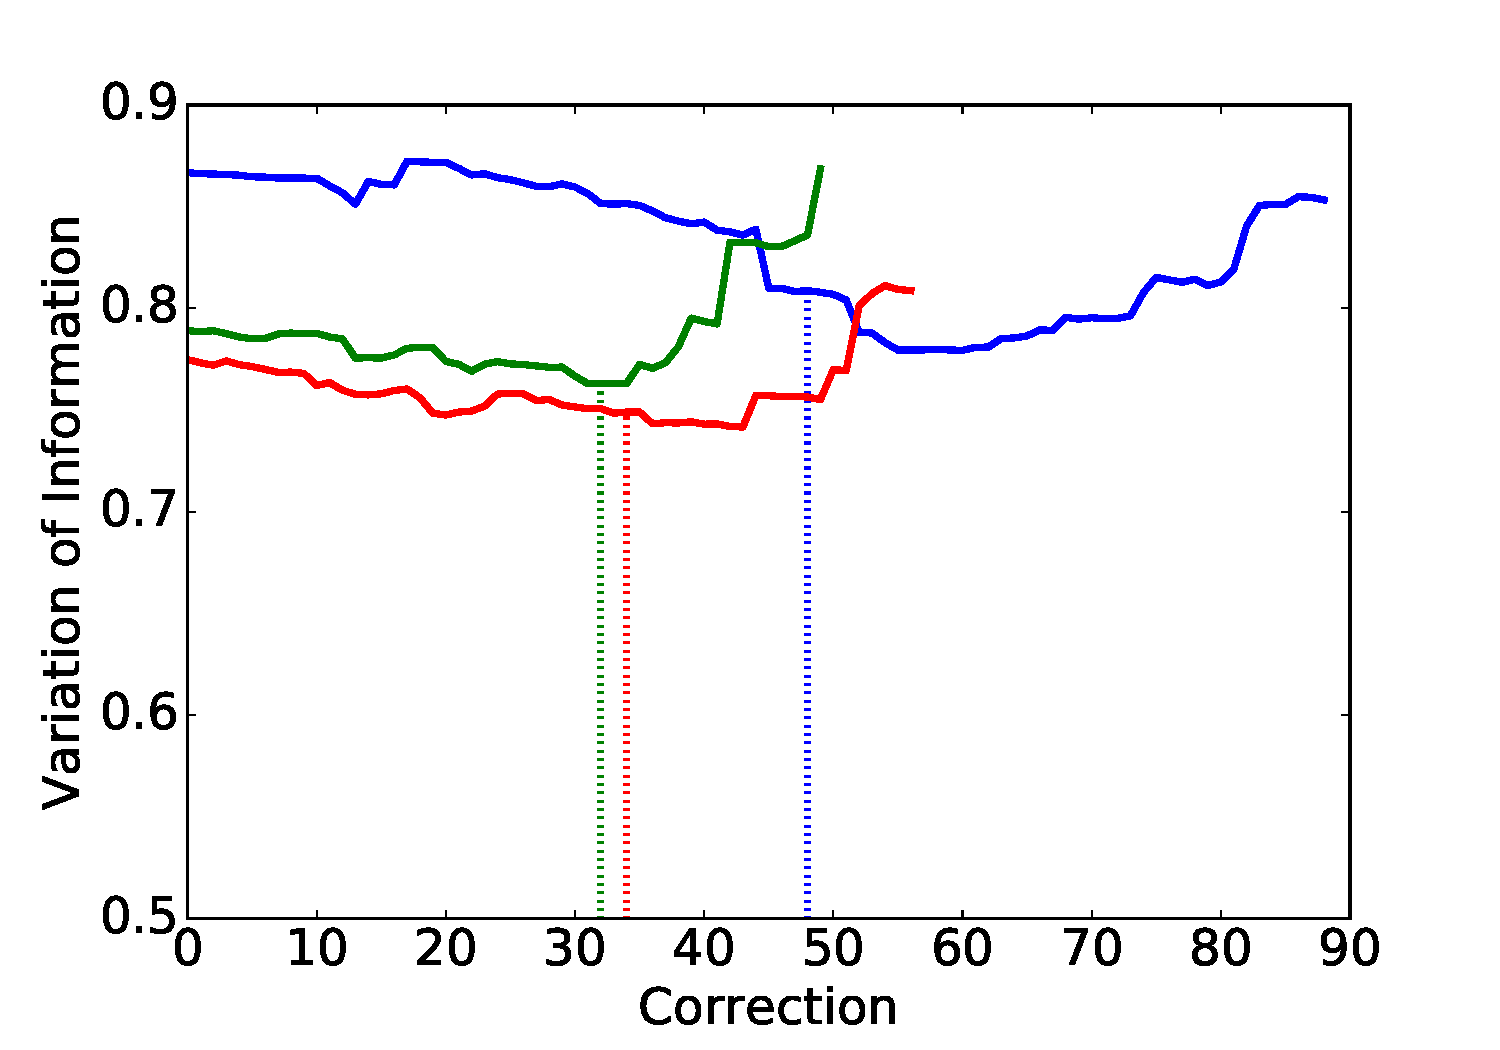
\includegraphics[width=\linewidth]{gfx/ptplot.pdf}
\caption{Observations of probability thresholds $p_t$ during automatic selection on three different subvolumes of previously unseen testing data. The dashed lines show when $p_t=0.95$ is reached.}
\label{fig:cylboxplot}
\end{figure}

\subsection{Merge Error Detection Pseudo Code}

\begin{algorithm}[H]
\caption{Merge Error Detection for a label \emph{l}}\label{code:mergeerror}
\begin{algorithmic}[1]
%\State{mergeErrors = []}
%\For{\emph{l} in $\forall$labels}
	\State{$l_d$ = \textbf{dilate}(\emph{l}, 20)}
	\State{invImage = \textbf{invert}(image)}
	\For{N iterations}
		\State{$s_1$, $s_2$ = \textbf{randomSeedsOnBoundary}($l_d$)}
		\State{wsImage = \textbf{watershed}(invImage, $l_d$, $s_1$, $s_2$)}
		\State{border = \textbf{border}(wsImage)}
		\State{$p$ = \textbf{rank}(border)}
		\State{$p_\text{merge}$ = $1-p$}	
	\EndFor
	\State{\textbf{find}(max $p_\text{merge})$}

\end{algorithmic}
\end{algorithm}

\subsection{Limitations}
Guided proofreading works on 2D image sections. This enables error correction without a computationally expensive alignment process. However, the output requires an additional (block-)merging step prior to 3D analysis. Several software packages exist for this purpose.

As described in Section~\ref{sec:addexp}, the guided proofreading classifier has to be retrained if used on a different species than mouse. In our experiments, parameters did not need to be changed.

\section{Automatic Segmentation Pipeline}

We create a dense automatic segmentation of electron microscopy data using a combination of a U-net~\cite{RonnebergerFB15} and the GALA agglomeration method~\cite{nunez2014graph}. These classifiers are trained on different data than GP (Tab.~\ref{tab:trainingdata}).

\begin{table}[h]
\caption{Training data of membrane detection (U-Net / GALA) vs.~training data of GP vs.~test data.}%While the training of our classifier is more expensive, testing accuracy is superior. }
\vspace{-1mm}
\resizebox{\linewidth}{!}{
\begin{tabular}{lrrrr}
\toprule
%Dataset & \makecell{Training Set\\Membrane Detection (U-Net)} & \makecell{Training Set\\Guided Proofreading} \\ 
\makecell{Training Set\\U-Net / GALA} & \makecell{Training Set\\GP} & \makecell{Test Set\\GP}\\ 
\midrule
\makecell{AC3+AC4\\($1024\times1024\times175$vx)} & \makecell{L. Cylinder\\($2048\times2048\times250$vx)} &
\makecell{$\text{L. Cylinder}_\text{test}$\\($2048\times2048\times50$vx)}
\\ 
\makecell{AC4 excl. test\\ ($1024\times1024\times90$vx)} &  \makecell{L. Cylinder\\($2048\times2048\times250$vx)} &
\makecell{$\text{AC4}_\text{test}$ subvolume\\($400\times400\times10$vx)} \\ 
\makecell{AC3+AC4\\($1024\times1024\times175$vx)} & \makecell{CREMI A/B/C\\($1250\times1250\times300$vx)} &
\makecell{$\text{CREMI A/B/C}_\text{test}$\\($1250\times1250\times15$vx)} \\ 
\bottomrule
\end{tabular} 
}
\label{tab:trainingdata}
\end{table}

GALA uses a random forest classifier to agglomerate segments. We use an agglomeration level of 0.3 (after a grid search). Further details of our pipeline are described in~\cite{rhoananet}.